 \documentclass{beamer}

\usetheme{MagdeburgFIN}
\usefonttheme{structurebold}
\usepackage{graphicx}
\usepackage{float}
\usepackage{url}
\usepackage{pdfpages}
\usepackage{mathtools}
\usepackage{algorithm}
\usepackage{algorithmic}
\usepackage{caption}



\title{Computational Intelligence in Games}
\author{Emergence}
\date{\today}
\institute{Otto-von-Guericke-University Magdeburg}


\begin{document}


\begin{frame}[plain]
 \titlepage
\end{frame}

% Fred
\begin{frame}
\frametitle{Agenda}
\begin{itemize}
\item Dummy
\item Dummy
\item Dummy
\item Dummy
\item Dummy
\end{itemize}
\end{frame}


% Julian
\begin{frame}
\frametitle{Stay Alive Agent}
Stay Alive by using
\begin{itemize}
\item the advance() method multiple times
\item the grid observation
\item a combination of that approaches
\end{itemize}

\begin{figure}
\centering
\begin{minipage}{.5\textwidth}
  \centering
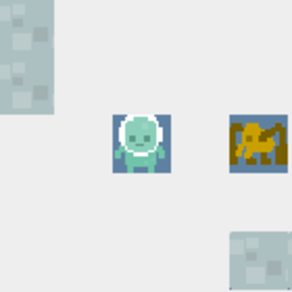
\includegraphics[scale=0.8]{../report/images/safe.pdf}
\caption{Advancing safe actions}
\label{fig:safe}
\end{minipage}%
\begin{minipage}{.5\textwidth}
\centering
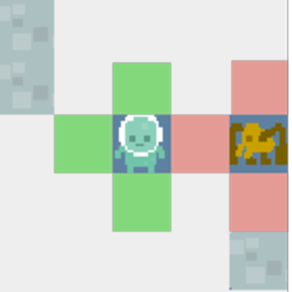
\includegraphics[scale=0.8]{../report/images/safe_grid.pdf}
\caption{Grid search for safe actions}
\label{fig:safe_grid}
\end{minipage}
\end{figure}



\end{frame}



% Julian
\begin{frame}
\frametitle{Heuristic Agent}
\begin{itemize}
\item Heuristic for selecting the next best step (including the Stay Alive Strategy)
\item Target is found by using an Explorer that is searching for
the point of interests

\item An Environment class builds up the knowledge base and safes
blocking, loosing, scoring and winning objects

\item A* Algorithm is used to reached the good classified objects

\end{itemize}

\begin{figure}
\centering
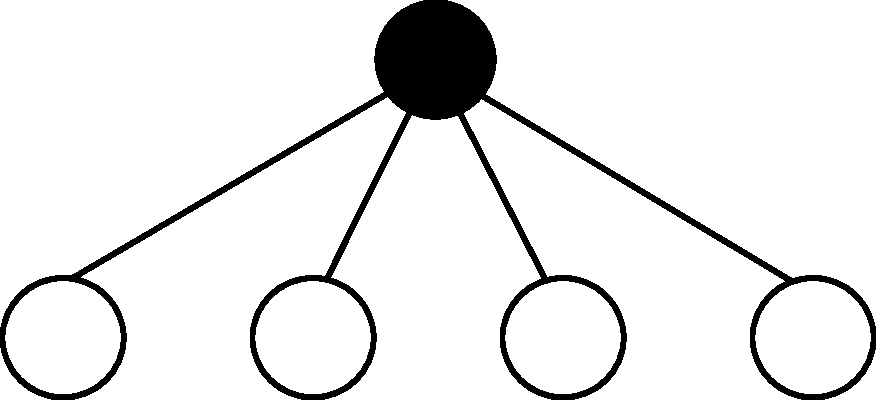
\includegraphics[scale=0.3]{../report/images/onestep_lookahead.pdf}
\caption{Search tree for the greedy approach}
\label{fig:onestep}
\end{figure}

\end{frame}



\begin{frame}
\frametitle{Heuristic Agent II}
\begin{equation}
dist(u,v) = |x_{1} - x_{2}| + |y_{1} - y_{2}|
\end{equation}
\begin{figure}
\centering
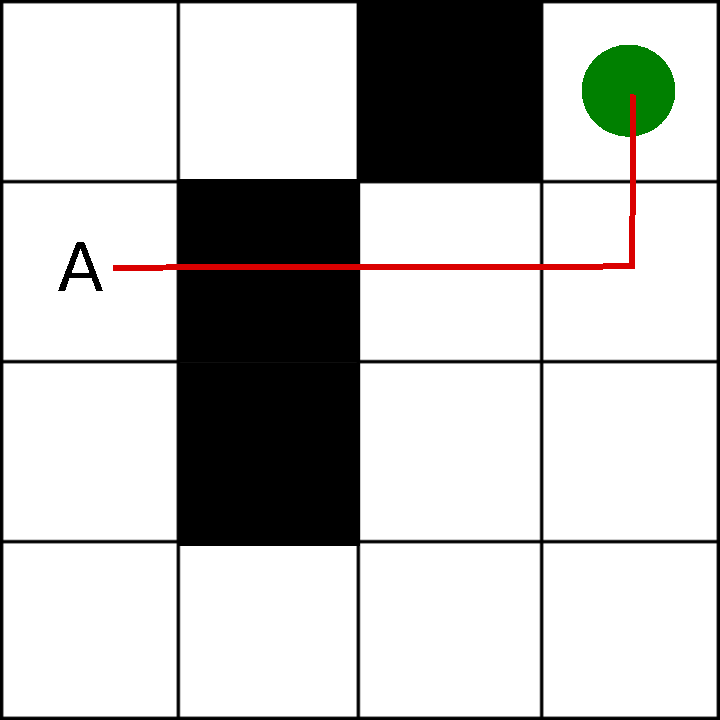
\includegraphics[scale=0.3]{../report/images/manhatten.pdf}
\caption{Manhatten distance for two dimensions}
\label{fig:manhatten}
\end{figure}
\end{frame}





% Fred
\begin{frame}
\frametitle{MCTS}
\begin{itemize}
 \item Dummy
\end{itemize}
\end{frame}

\begin{frame}
\frametitle{MCTS Agent}
\begin{itemize}
 \item Dummy
\end{itemize}
\end{frame}

\begin{frame}
\frametitle{MCTS Agent II}
\begin{itemize}
 \item Dummy
\end{itemize}
\end{frame}


% Julian
\begin{frame}
\frametitle{EA}



\begin{algorithm}[H]
\caption{Pseudocode of an evolutionary algorithm }
\begin{algorithmic}[1]

\STATE \emph{Initialize} Population with random candidate solutions;
\STATE \emph{Evaluate} each candidate;
\WHILE{Termination condition not satisfied} 
\STATE \emph{Select} parents 
\STATE \emph{Recombine} pairs of parents
\STATE \emph{Mutate} the resulting offspring
\STATE \emph{Evaluate} new candidates
\STATE \emph{Select} individuals for the next generation
\ENDWHILE

\end{algorithmic}

\label{alg:seq}
\end{algorithm}


\end{frame}





\begin{frame}
\frametitle{EA Agent}

DeltaScoreEvaluation function 
\begin{equation*}
s = \sum_{t=0}^n (H(s_t) - H(s_{t-1}))
\end{equation*}

is calculated by using the function

\begin{equation*}
    H(s_i, s_{i-1}) = 
\begin{dcases}
    10, & \text{if isWinner}  \\
    -10, & \text{if isLooser}  \\
    score(s_i) - score(s_{i-1}), & \text{otherwise.}
\end{dcases}
\end{equation*}
\end{frame}



\begin{frame}
\frametitle{EA Agent II}
\begin{figure}[H]
\centering
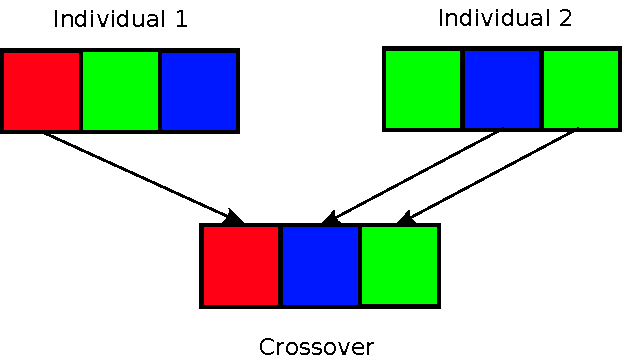
\includegraphics[scale=0.6]{../report/images/crossover.pdf}
\caption{Crossover of an individual}
\label{fig:crossover}
\end{figure}
\end{frame}


\begin{frame}
\frametitle{EA Agent III}
\begin{figure}[H]
\centering
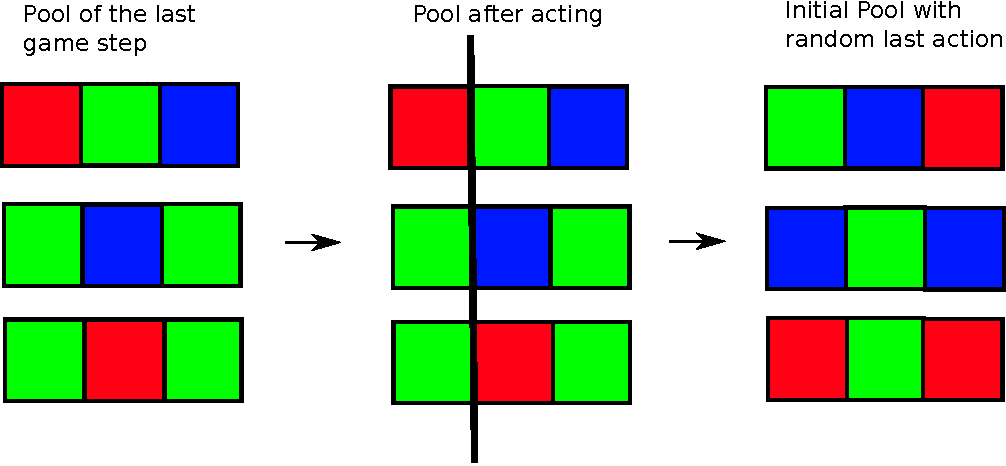
\includegraphics[scale=0.6]{../report/images/sliding_window.pdf}
\caption{Sliding Window}
\label{fig:sliding_window}
\end{figure}
\end{frame}


% Julian
\begin{frame}
\frametitle{Experiment Result}
\begin{itemize}
\item Comparison among each approach to be fair (1000 games, one game 50 times, 10 times each level)
\item Evaluation of the best of each algorithm (3000 games, one game 150 times, 30 times each level)
\end{itemize}

\begin{table}
\center
\begin{tabular}{ll} 
\textbf{CPU} & Intel i5-4210U @ 1.70Ghz \\ \hline
\textbf{Memory} & 8 GB DDR3 L \\  \hline
\textbf{Operating System} & Ubuntu 14.04.1 LTS \\  \hline
\textbf{Java Version} &  1.7.0\_65\\  
\end{tabular}
\caption{experiment setup}
\end{table}
\end{frame}



\begin{frame}
\frametitle{Experiment Result II}
\begin{table}
\center
\begin{tabular}{c|c|c|c|c|c|c|c|c|}  \hline
\multicolumn{1}{p{1.4cm}|}{\centering \\ Approach} & 
\multicolumn{1}{p{1cm}|}{\centering Avg \\ Wins	} & 
\multicolumn{1}{p{1cm}|}{\centering Std \\ Wins} &
\multicolumn{1}{p{1cm}|}{\centering Avg \\ Score	} & 
\multicolumn{1}{p{1cm}|}{\centering Std \\ Score} &
\multicolumn{1}{p{1cm}|}{\centering Avg \\ time \\ steps 	} & 
\multicolumn{1}{p{1cm}|}{\centering Std \\ time \\ steps} \\ \hline
HR & \textbf{0.527} & 0.029 & 165.05 & 59.51 & \textbf{695.86} & 36.17 \\ \hline
MCTS & 0.467 & 0.034 & \textbf{230.69} & 74.64 & 942.06 & \textbf{34.00} \\ \hline
EA & 0.470 & \textbf{0.026} & 178.33 & \textbf{51.85} & 818.72 & 38.47 \\ \hline
\end{tabular}
\caption{results of all algorithms}
\label{tbl:all_result}
\end{table}

\end{frame}



\begin{frame}
\frametitle{Experiment Result III}
\begin{figure}[H]
\centering
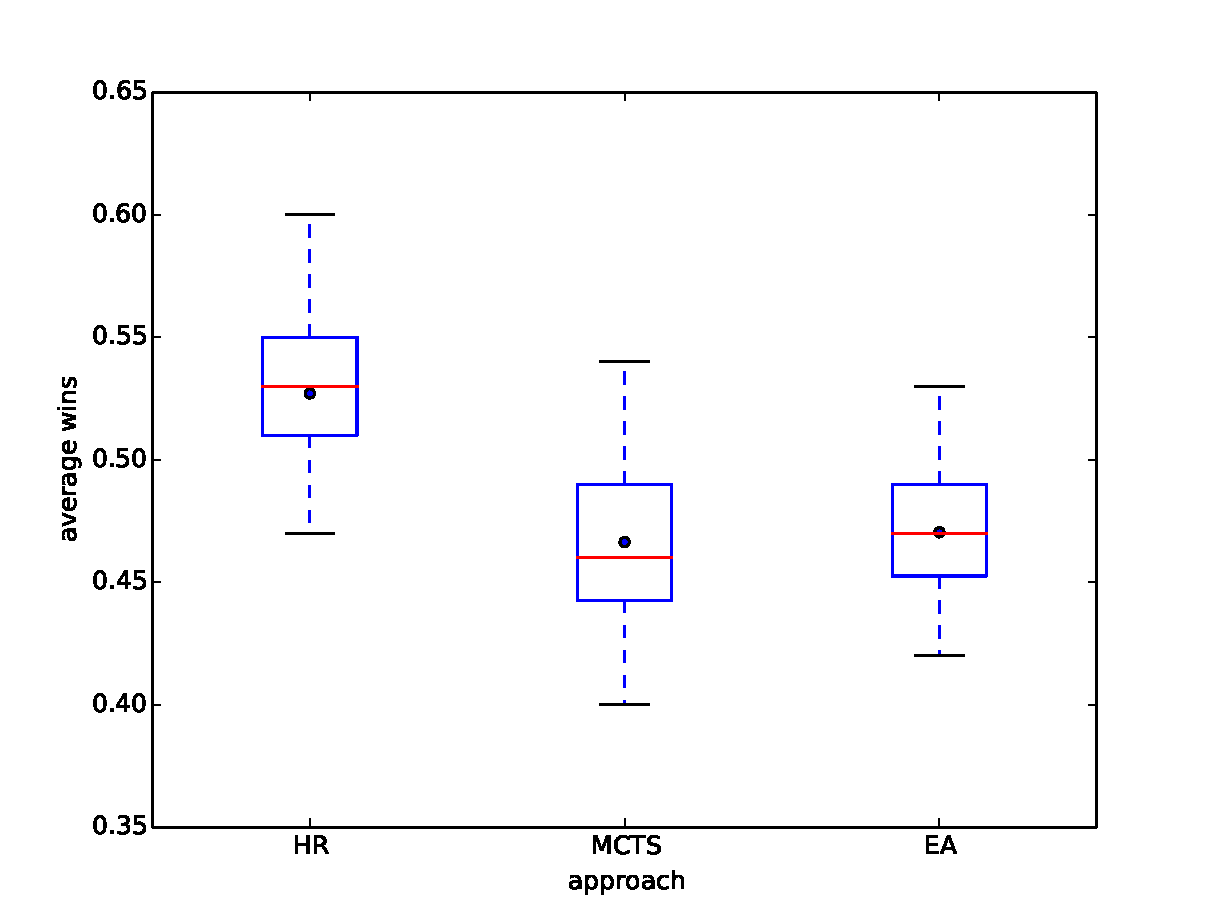
\includegraphics[scale=0.45]{../report/images/eval_all_wins.pdf}
\caption{boxplot of wins}
\label{box_eval_all_wins}
\end{figure}
\end{frame}



% Fred
\begin{frame}
\frametitle{Development Process}
\begin{itemize}
 \item Dummy
\end{itemize}
\end{frame}


\begin{frame}
\frametitle{Main Problems Difficulties}
\begin{itemize}
 \item Dummy
\end{itemize}
\end{frame}


\begin{frame}
\frametitle{Conclusion \& Future Work}
\begin{itemize}
 \item Dummy
\end{itemize}
\end{frame}




\begin{frame}
\begin{center}
\textbf{\LARGE Thank you for your attention!}
\end{center}

\end{frame}


\end{document}
